\documentclass[11pt]{article}
\renewcommand{\baselinestretch}{1.2}
\usepackage[utf8]{inputenc}
\usepackage{amsmath}
\usepackage{caption}
\usepackage{subcaption}
\usepackage{graphicx} %package to manage images
\graphicspath{ {Images/} }
\usepackage{xcolor}
\usepackage{makeidx}
\definecolor{dkgreen}{rgb}{0,0.6,0}
\definecolor{gray}{rgb}{0.5,0.5,0.5}
\definecolor{mauve}{rgb}{0.58,0,0.82}
\usepackage{listings}
\usepackage[T1]{fontenc} % Output font encoding for international characters
\usepackage[margin=1.2in]{geometry}

\usepackage{amsmath}
\usepackage{mathpazo} % Palatino font
% \usepackage[style=authoryear,backend=biber]{biblatex}
\lstset{frame=tb,
  language=Matlab,
  aboveskip=3mm,
  belowskip=3mm,
  showstringspaces=false,
  columns=flexible,
  basicstyle={\small\ttfamily},
  numbers=none,
  numberstyle=\tiny\color{gray},
  keywordstyle=\color{blue},
  commentstyle=\color{dkgreen},
  stringstyle=\color{mauve},
  breaklines=true,
  breakatwhitespace=true,
  tabsize=3
}

\usepackage[
    backend=biber,
    style=numeric,
		sorting=none,
    natbib=true,
    url=false,
    doi=true,
    eprint=false
]{biblatex}
\addbibresource{references.bib}
\begin{document}


\begin{titlepage} % Suppresses displaying the page number on the title page and the subsequent page counts as page 1
	\newcommand{\HRule}{\rule{\linewidth}{0.5mm}} % Defines a new command for horizontal lines, change thickness here
	
	\center % Centre everything on the page
	
	%------------------------------------------------
	%	Headings
	%------------------------------------------------
	
	\textsc{\LARGE Imperial College London}\\[1.5cm] % Main heading such as the name of your university/college
	
	\textsc{\Large Electrical and Electronic Engineering Department}\\[0.5cm] % Major heading such as course name
	
	%------------------------------------------------
	%	Title
	%------------------------------------------------
	
	\HRule\\[0.4cm]
	
	{\huge\bfseries Interim Report}\\[0.4cm] % Title of your document
	
	\HRule\\[1.5cm]
	
	%------------------------------------------------
	%	Author(s)
	%------------------------------------------------
	
	
	% If you don't want a supervisor, uncomment the two lines below and comment the code above
	{\large\textit{Project title}}\\
	\textsc{Structure and dynamics of large networks of interacting neurons}
	
	\vfill
	%------------------------------------------------
	%	Author(s)
	%------------------------------------------------
	
	
	% If you don't want a supervisor, uncomment the two lines below and comment the code above
	{\large\textit{Author}}\\
	\textsc{Alejandro Gilson Campillo} \quad \text{CID: 01112712} % Your name
	
	\vfill
	%------------------------------------------------
	%	Supervisor
	%------------------------------------------------
	
	
	{\large\textit{Supervisor}}\\
	\textsc{Prof. Pier Luigi Dragotti} 
	%------------------------------------------------
	%	Second Marker
	%------------------------------------------------
	
	\vfill
	
	{\large\textit{Second Marker}}\\
	\textsc{Dr. Wei Dai} 
	%------------------------------------------------
	%	Date
	%------------------------------------------------
	\vfill\vfill\vfill % Position the date 3/4 down the remaining page
	
	{\large\today} % Date, change the \today to a set date if you want to be precise
	
	%------------------------------------------------
	%	Logo
	%------------------------------------------------
	
	\vfill\vfill
	 
	
\includegraphics[width=5cm]{imperialcollegelondon.jpg}\\[1cm] % Include a department/university logo - this will require the graphicx package	
	%----------------------------------------------------------------------------------------
	
	\vfill % Push the date up 1/4 of the remaining page
	
\end{titlepage}

\begin{titlepage}
\tableofcontents
\end{titlepage}

\section{Introduction}

The brain is a complex machine, it allows the human being to think, communicate and feel. It does so thanks to the billions of neurons that communicate in a dense network through synapses. However, little is known about how it works. By studying how the neurons structure to store and process information we can understand how the brain as a whole functions. This could have important applications in medicine for curing diseases such as Parkinson \cite{OldeDubbelinkKimT.E.2014Dbnt} and epilepsy \cite{PONTEN2007918}, and in machine learning for the development of more intelligent neural networks.
\\\\
In order to infer the network structure of a set of neurons, they are treated as a diffusion network where electrical spikes increase the likelihood of connected neurons to spike and therefore transmit a signal that travels as if it were a disease. By evaluating the time of "infection", the relationship between two neurons can be probabilistically estimated. After computing the relationship between all of the neurons, an estimate of the topology of the network can be obtained. 
\\\\
Previous work on this topic \cite{pranav_report, alexandru2018estimating} evaluated the feasibility of using a maximum-likelihood estimator algorithm, NetRate \cite{rodriguez2011uncovering}, for the structure inference of biological neural networks. A network was simulated using the Izhikevic neuron model \cite{izhikevich2003simple} and the brian simulator \cite{10.3389/neuro.01.026.2009}. The connections between the neurons were then estimated, compared to the original network and the performance of the algorithm was evaluated.
\\
\\
The aim of this project is to improve on the state of the art research of network inference and the understanding of the underlying structure of the brain. There are many ways in which this can be done such as scalability and the addition of different types of neurons to the model.It would also be useful to test the accuracy of the algorithm on real interacting neurons. Developments in technology allow us to obtain spike data from individual neurons \cite{ito2016spontaneous, ito2014large, litke2004does}.


\section{Background}

\subsection{Definition of connectivity}

The definition of connectivity between neurons has a history of lack of consensus among the scientific community \cite{HORWITZ2003466}. Connectivity studies from different researchers may lead to different results depending on how they define it, as they may be looking at different aspects of connectivity. The two main accepted definitions that are used are functional and effective connectivity.
\\
Functional connectivity is the temporal correlation between spatially remote neurophysiological events \cite{friston1993functional}. Studies on this topic began with electroencephalography (EEG) measurements. Some methods to measure functional connectivity include the evaluation of the correlation in the frequency domain between EEG signals at different scalp locations \cite{pfurtscheller1999event}, and the cross-correlation of the time series measurements from a pair of electrodes \cite{gevins1985neurocognitive}. However, due to the volume conduction of brain tissue, the electrical activity from the scalp cannot infer the individual neuron behaviour below the electrode \cite{HORWITZ2003466}.
\\
Effective connectivity was defined in \cite{friston1993functional} as the influence that one neural system exerts on another. Effective connectivity can be measured in terms of efficacy and contribution. At a synaptic level it can be expressed as in Eq.\ref{eq:synaptic_effectivity}, where $x_{j}$ is the post-synaptic response to many pre-synaptic inputs $x_{i}$ and $\textbf{W}_{ij}$ is the efficacy of the connections between neurons $i$ and $j$. Contribution is reflected in Eq.\ref{eq:synaptic_contribution} as the effect of $i$ on $j$ relative to all pre-synaptic inputs. Using this definition, directional effects are taken into account and a richer representation of the network can be attained. Following the approach in \cite{alexandru2018estimating}, this project will focus on the effective connectivity of neurons in a network.
\\

\begin{equation}\label{eq:synaptic_effectivity}
x_{j} = \Sigma \textbf{W}_{ij}\times x_{i}
\end{equation}

\begin{equation}\label{eq:synaptic_contribution}
\frac{\textbf{W}_{ij}}{\Sigma \textbf{W}_{ij}}
\end{equation}

\subsection{Izhikevich neuron model}

In order to understand how the brain works we must be able to replicate the behaviour of individual neurons applying simple and accurate models. However, as explained in \cite{izhikevich2003simple}, meeting both criteria can be challenging. The Hodgkin–Huxley model \cite{hodgkin1952quantitative} is very accurate as it can emulate the rich firing patterns of many types of neurons. However, it is very computationally expensive and only a few neurons can be computed in real time. The integrate-and-fire model \cite{burkitt2006review}  has the opposite problem: it is computationally simple but it is an unrealistic representation of the neuron since it does not capture the firing patterns with sufficient accuracy \cite{izhikevich2003simple}.
\\
In contrast, the Izhikevich neuron model \cite{izhikevich2003simple} meets both criteria. Tens of thousands of spiking cortical neurons can be simulated in real time by simplifying the Hodgkin-Huxley model into the two dimensional system of differential equations shown below.


\begin{align}\label{eq:izhikevich_ode}
&v'=0.04v^{2}+5v+140-u+\textbf{I} \\
&u'=a(bv-u)
\end{align}

with the auxiliary after-spike reseting

\begin{equation}\label{eq:izhikevich_reset}
\text{if } v \geq 30 \text{mV, then}
\begin{cases}
    v     & \leftarrow c \\
    u     & \leftarrow u + d 
  \end{cases}
\end{equation}

Here, the dimensionless variables $v$ and $u$ represent the membrane potential of the neuron and the membrane recovery, respectively. When a spike reaches its apex (30 mV), both these variables are reset according to Eq. \ref{eq:izhikevich_reset}. Synaptic or injected DC currents are represented by the variable \textbf{I}. The threshold is not fixed, just as with real neurons and it's based on previous spikes. 
\\
On the other hand, $a, b, c$ and $d$ are dimensionless parameters. $a$ determines the speed of the recovery variable $u$, $b$ defines the sensitivity of the recovery variable $u$ to sub-threshold fluctuations of the membrane potential $v$. Finally, $c$ and $d$ determine the after-spike reset value of the recovery variables $v$ and $u$, respectively. 
\\
The relevance of this algorithm stems from the fact that, different combinations of the parameters provide the model with a rich variety of firing patterns. When analysing the neocortical neurons in the mammalian brain, a number of different classes of excitatory neurons can be found \cite{connors1990intrinsic, gray1996chattering} such as RS (regular spiking), IB (intrinsically bursting) and CH (chattering). From the inhibitory type of neurons, two classes can be found: FS (fast spiking and LTS (low-threshold spiking). Other interesting classes of neurons are the TC (thalamo-cortical) and the RZ (resonator). A visual representation of these neurons can be observed in figure \ref{fig:types_neurons}. It is of great importance to understand what types of neurons can be found so that a simulated network can become a closer representation of what can be found on a real brain. In order to simplify the network to be inferred, the only type of neurons simulated in the network were the excitatory regular spiking neurons. This was achieved by setting the parameters to $a=0.02$, $b=0.2$, $c=-65$ and $d=8$. This type of neuron is the most common type of excitatory neuron in the brain. There is also a ratio of excitatory and inhibitory neurons of 4 to 1 in the mammalian brain, respectively \cite{izhikevich2003simple}.

In order to make use of the Izhikevich neuron model, Eq.\ref{eq:izhikevich_ode} is declared in the Brian Simulator. This library computes the membrane potential voltage of the interacting neurons in the network and outputs all of their spiking times. This data will then be used to compute the NetRate algorithm.


\begin{figure}
	\label{fig:types_neurons}
  \centering
	\begin{subfigure}[b]{0.49\textwidth}
		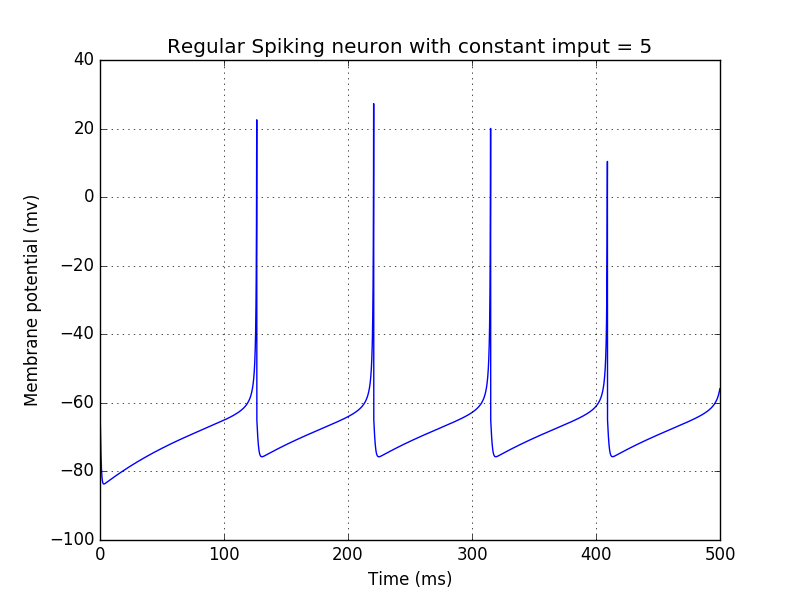
\includegraphics[width=\textwidth]{regular_spiking.png}
	\end{subfigure}
	\begin{subfigure}[b]{0.49\textwidth}
		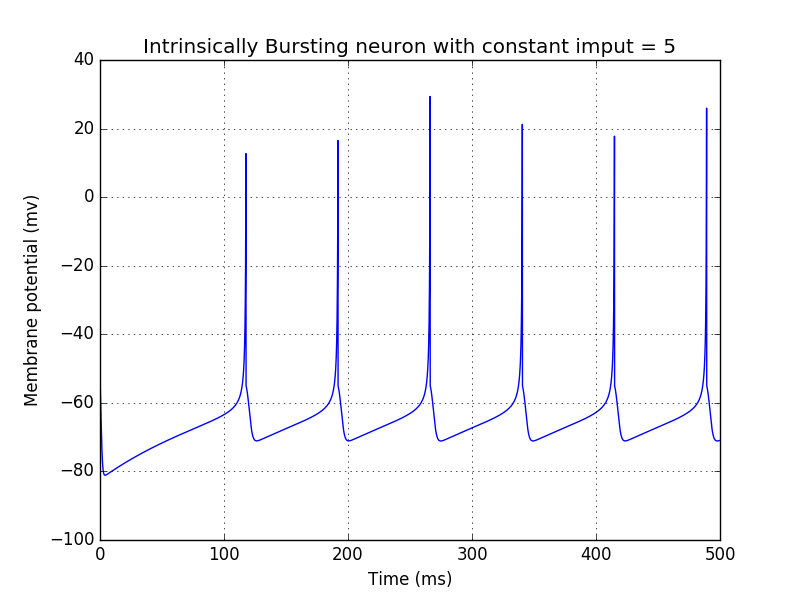
\includegraphics[width=\textwidth]{intrinsically_bursting.png}
	\end{subfigure}
	\begin{subfigure}[b]{0.49\textwidth}
		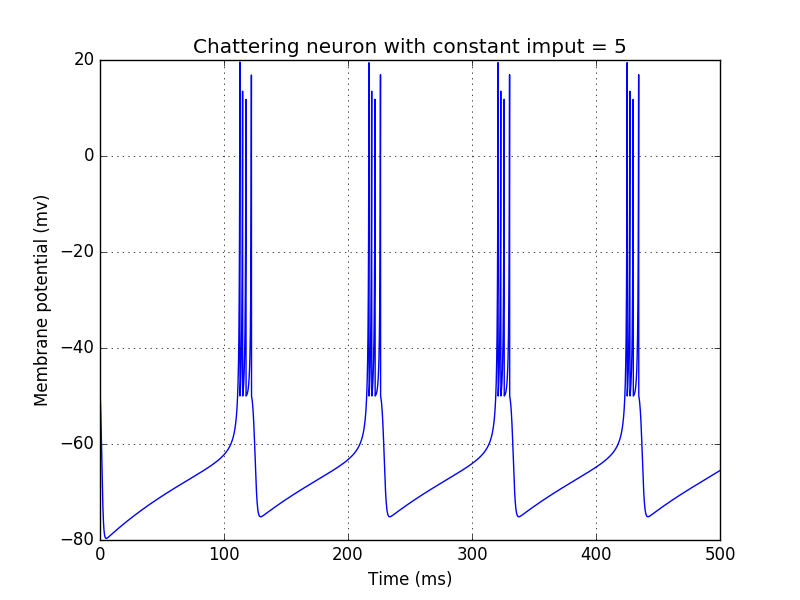
\includegraphics[width=\textwidth]{chattering.png}
	\end{subfigure}
	\begin{subfigure}[b]{0.49\textwidth}
		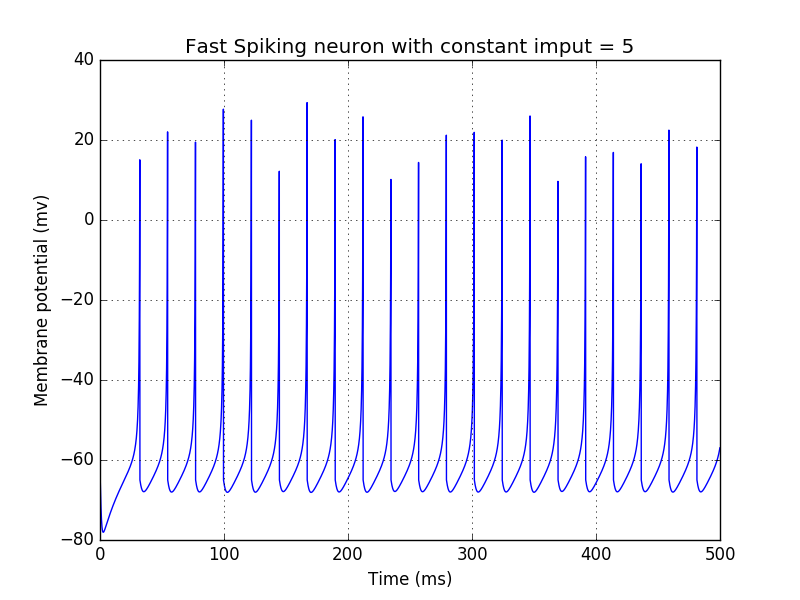
\includegraphics[width=\textwidth]{fast_spiking.png}
	\end{subfigure}
  \caption{Types of neurons in the mammalian brain. Generated with the Brian Simulator \cite{10.3389/neuro.01.026.2009} using the Izhikevich neuron model \cite{izhikevich2003simple}}
\end{figure}


\subsection{Netrate}

\subsubsection{Diffusion processes}\label{sec:diffusion_processes}

In order to infer the underlying structure of a network, \cite{alexandru2018estimating} employed  NetRate algorithm developed by Rodriguez \cite{rodriguez2011uncovering} by treating the network as a diffusion process.

The study of diffusion network is based on the observation of the nodes in a system when they take a certain action: get infected by a virus, share a piece of information, etc. A problem concerning this kind of studies lies on the fact that we can only understand when and where these nodes propagate but not how or why the do so. An example of this is the propagation of a virus in a population. We can tell who and when somebody got infected but not who infected him. For the rest of this section we will refer to the propagation of an infection as the object of study of the network. 

To infer the mechanisms behind diffusion processes the time of infection is analysed. A model needs to be created with some assumptions about the structures that generate diffusion processes:

\begin{itemize}
\item The network in a diffusion process is fixed, unknown and directed.
\item Infections are binary, they can only be infected or not infected, no partial infections are considered.
\item Infections across the edges of the network occur independently from one another.
\item The likelihood of a node $a$ infecting node $b$ at time $t$ is modelled by a probability distribution dependent on $a, b$ and $t$.
\item All infections in a network are observed during a recorded time window.
\end{itemize}

NetRate aims to describe how infections occur during a period of time in a fixed network. This is achieved by finding the optimal network and transmission rates that maximizes the likelihood of a set of observed cascades to occur. The mathematical definitions that construct this model will be explained in the following section.


\subsubsection{Mathematical definitions}

The following definitions in this section are necessary for the construction of the model with which we intend to infer the connectivity of the network. First, the data that is going to be analysed will be defined:

\begin{itemize}
\item Observations are carried out on a population of $N$ nodes that have created a set of $C$ cascades $\{\textbf{t}^{1},\cdots,\textbf{t}^{|C|}\}$. 
\item Each of the cascades $\textbf{t}^{c}$ contains the infection times of all the population within a time period $T^{c}$.
\item Each of the cascades is an N-dimensional vector with recordings of when the nodes were infected in the cascade. If a node was not infected during the time period $[0,T^{c}]$, a symbol $\infty$ is assigned. This does not mean that the node never gets infected.
\begin{equation}\label{eq:data_netrate}
\textbf{t}^{c}:=(t_{1}^{c},\cdots,t_{N}^{c}),\quad t_{k}^{c}\in [0,T^{c}]\cup{\infty}
\end{equation}
\item For simplicity, $T^{c}=T$
\item Node $i$ is parent of node $j$ if $t_{i}<t_{j}$ within the cascade.
\end{itemize}

The pairwise interactions are to be studied in order to obtain the pairwise transmission likelihood between nodes in the network. It will be assumed that infections can occur at different rates along different edges in the network. 

\begin{itemize}
\item $f(t_{i}|t_{j},\alpha _{j,i})$ is the conditional likelihood of transmission between nodes $j$ and $i$. It depends on the infection times $(t_{i},t{j})$ and pairwise transmission rate $\alpha_{j,i}$.
\item A node cannot be infected by a healthy node. Node $j$, infected at $t_{j}$, can only infect node $i$ at time $t_{i}$ if and only if $t_{j}<t_{i}$.
\item Transmission rate $\alpha _{j,i}\geq0$.
\end{itemize}

The cumulative density function is defined as $F(t_{i}|t_{j};\alpha _{j,i})$ and is obtained from the transmission likelihood. If a node $j$ was infected at time $t_{j}$, the probability that node $i$ is not infected by node $j$ by time $t_{i}$ is given by the survival function of the edge $j\rightarrow i$:

\begin{equation}\label{eq:survival_function}
S(t_{i}|t_{j};\alpha _{j,i})=1-F(t_{i}|t_{j};\alpha _{j,i})
\end{equation}

The instantaneous infection rate, or hazard function, of the edge $j\rightarrow i$ is the ratio of the transmission likelihood over the survival function as shown in Eq.\ref{eq:hazard_function}.

\begin{equation}\label{eq:hazard_function}
H(t_{i}|t_{j};\alpha _{j,i})=\frac{f(t_{i}|t_{j};\alpha _{j,i})}{S(t_{i}|t_{j};\alpha _{j,i})}
\end{equation}

With a complete set of definitions, it will now be possible to derive the algorithm behind NetRate as it will be shown in the next section.

\subsubsection{Derivation of NetRate}

Rodriguez \cite{rodriguez2011uncovering} derives NetRate by studying the individual probability of infection of the nodes and then building the whole of the network. The probability of survival of any cascade is the probability that a node is not infected until time $T$, given that the parents are infected at the beginning of the cascade. For a non-infected node $i$, the probability that any of the nodes $1\cdots N$ does not infect node $i$ by time $T$ is given by the product of the survival functions of each of the infected nodes $k$ targeting node $i$ because the different probabilities of infection are considered independent. This is illustrated in Eq.\ref{eq:step_1_netrate}.

\begin{equation}\label{eq:step_1_netrate}
\prod_{t_{k}\leq T}S(T\mid t_{k};\alpha _{k,i})
\end{equation}

To compute the likelihood of a cascade $\textbf{t}:=(t_{1},\cdots,t_{N}|t_{i}\leq T)$ we require the the likelihood of the recorded infections $\textbf{t}^{\leq T}=(t_{1},\cdots,t_{N}|t_{i}\leq T)$. Again, using independence, the likelihood factorizes as seen in \ref{eq:step_2_netrate}. The likelihood of the cascade then becomes the conditional likelihood of the infection time given the rest of the cascade.

\begin{equation}\label{eq:step_2_netrate}
f(\textbf{t}^{\leq T};\textbf{A})=\prod_{t_{i}\leq T}f(t_{i}\mid t_{1},\cdots,t_{N}\backslash t_{i};\textbf{A})
\end{equation}

As in \cite{kempe2003maximizing}, a node gets infected when the first parent infects the node. We now compute the likelihood of a potential parent $j$ of being the first one by using Eq.\ref{eq:step_1_netrate}.

\begin{equation}\label{eq:step_3_netrate}
f(t_{i}\mid t_{j};\alpha_{j,i})\times \prod_{j\neq k,t_{k}< t_{i}}S(t_{i}\mid t_{k};\alpha _{k,i})
\end{equation}
 
In this step, we calculate the conditional likelihood of Eq.\ref{eq:step_2_netrate} by adding all the likelihoods of the mutually disjoint likelihoods that each potential parent is the first parent:

\begin{equation}\label{eq:step_4_netrate}
f(t_{i}\mid t_{1},\cdots,t_{N}\backslash t_{i};\textbf{A})=\sum_{j:t_{j}<t_{i}}f(t_{i}\mid t_{j};\alpha _{j,i})\times \prod _{j\neq k,t_{k}<t_{i}}S(t_{i}\mid t_{k};\alpha _{k,i})
\end{equation}

Using Eq.\ref{eq:step_2_netrate} and removing the condition $k\neq j$, the likelihood of infections then becomes:

\begin{equation}\label{eq:step_5_netrate}
f(\textbf{t}^{\leq T};\textbf{A})=\prod_{t_{i}\leq T}\prod_{k:t_{k}<t_{i}}S(t_{i}\mid t_{k};\alpha _{k,i})\times \sum_{j:t_{j}<t_{i}}\frac{f(t_{i}\mid t_{j};\alpha_{j,i})}{S(t_{i}\mid t_{j};\alpha _{j,i})}
\end{equation}

However, Eq.\ref{eq:step_5_netrate} needs to consider also the nodes that are not infected during the observation window. For this reason we add the multiplicative survival term from Eq.\ref{eq:step_1_netrate} and replace the ratios from Eq.\ref{eq:step_5_netrate} with hazard functions:

\begin{equation}\label{eq:step_6_netrate}
f(\textbf{t};\textbf{A})=\prod_{t_{i}\leq T}\prod_{t_{m}>T}S(T\mid t_{i};\alpha_{i,m})\times \prod_{k:t_{k}<t_{i}}S(t_{i}\mid t_{k};\alpha _{k,i})\sum_{j:t_{j}<t_{i}}H(t_{i}\mid t_{j};\alpha _{j,i})
\end{equation}

The likelihood of a set of independent set of cascades $C=\{t^{1},\cdots,t^{|C|}\}$ is the product of the likelihoods of all the individual cascades given by Eq.\ref{eq:step_6_netrate}:

\begin{equation}\label{eq:step_7_netrate}
\prod _{\textbf{t}^{c}\in C}f(\textbf{t}^{c};\textbf{A})
\end{equation}

The goal of the algorithm is to find the transmission rates $\alpha_{j,i}$ of all the edges in the network such that the likelihood of the set of cascades is maximized.

\begin{subequations}
\label{eq:optimization_netrate}
\begin{align}
& \text{minimize}_{\textbf{A}} -\sum_{c\in C}\log f(\textbf{t};\textbf{A})\\
& \text{subject to } \alpha _{j,i}\geq 0,i,j=1,\cdots,N,i\neq j,
\end{align}
\end{subequations}.

Here, $\textbf{A}:=\{\alpha _{j,i}\mid i,j=1,\cdots,n,i\neq j\}$ are the variables and the edges of the network are defined as the pairs of nodes whose transmission rates $\alpha _{i,j}>0$. 

The solution to Eq.\ref{eq:optimization_netrate} found in \cite{rodriguez2011uncovering} is given by \ref{eq:solution_netrate}. The survival and hazard functions are concave in the parameter(s) of the transmission likelihoods and, therefore, convexity of Eq.\ref{eq:optimization_netrate} follows from linearity. The network inference problem from Eq.\ref{eq:optimization_netrate} is thus convex for Power-Law, Rayleigh and Exponential models of the likelihood function.

\begin{subequations}
\begin{align}
\label{eq:solution_netrate}
& L(\{\textbf{t}^{1}\cdots \textbf{t}^{|C|}\};\textbf{A})=\sum _{c}\Psi_{1}(\textbf{t}^{c};\textbf{A})+\Psi_{2}(\textbf{t}^{c};\textbf{A})+\Psi_{3}(\textbf{t}^{c};\textbf{A})\\
& \Psi_{1}(\textbf{t};\textbf{A})=\sum _{i:t_{i}\leq T}\sum _{t_{m}>T}\log S(T\mid t_{i};\alpha _{i,m})\\
& \Psi _{2}(\textbf{t}^{c};\textbf{A})=\sum_{i:t_{i}\leq T} \sum_ {j:t_{j}<t_{i}}\log S(t_{i}\mid t_{j};\alpha_{j,i})\\
& \Psi _{3}(\textbf{t}^{c};\textbf{A})=\sum_{i:t_{i}\leq T} \log (\sum_{j:t_{j}<t_{i}} H(t_{i}\mid t_{j};\alpha_{j,i}))
\end{align}
\end{subequations}

The terms in Eq.\ref{eq:solution_netrate} depend only on the infection time differences ($t_{i}-t_{j}$) and the transmission rates $\alpha_{j,i}$. Each of the terms adds a property to the solution of NetRate.

\begin{itemize}
\item The terms $\Psi_{1}$ and $\Psi_{2}$ apply a positively weighted norm on $\textbf{A}$, thus encouraging sparse solutions.
\item $\Psi_{2}$ penalizes the edges that transmit infections slowly and promotes edges that infect quickly.
\item $\Psi_{1}$ penalizes edges to uninfected nodes until the time horizon. With a longer observation window the penalties become larger, but so does the probability of nodes becoming infected.
\item $\Psi_{3}$ makes sure that all infected nodes have a minimum of one parent to avoid $\log 0 = -\infty$. Since the logarithm grows slowly, it slightly encourages infected nodes to have many parents.
\end{itemize}

\subsubsection{Cascade generation}\ref{sec:cascade_generation}

The maximization of the likelihood function requires data in the form of cascades in order to be computed. The time of infection of each of the nodes can be obtained from the network simulation but it must then be formatted into cascades. The rest of this section is based on \cite{pranav_report}, where cascade generation is explained. 

\begin{enumerate}
\item At time $t=0$, a random node is selected to carry the disease.
\item The disease propagates for a $T$ amount of time (horizon) based on the pairwise transmission likelihood $f(t_{i}\mid t_{j};\alpha_{j,i})$ of the edges in the network.
\item At the end of the simulation, a cascade is generated with the information from the times at which the nodes were infected. 
\end{enumerate}

As an example, let there be a network of 6 nodes ($N=6$) and a horizon of $T=20$. Let us select node 5 at time $t=0$ to be the starting point of the experiment. The simulation begins and the disease spreads out. It infects node 2 at $t=3$ and node 6 at $t=5$. The resulting cascade has the form of Eq.\ref{eq:data_netrate}  would look like this:

\begin{equation}\label{eq:cascade_example}
\textbf{t}^{c}=\{\infty, 3, \infty, \infty, 0, 5\}
\end{equation}

In this cascade, nodes 2 and 6 were infected while nodes 1, 3 and 4 remained healthy for the duration of the cascade. Since at time $t=3$ the only infected node was 3, this node must have infected node 2. However, it becomes inconclusive as to which node infected 6 at time $t=6$. We could be lead to believe that the uninfected nodes are not connected to any of the other infected nodes. However, cascades are probabilistic models and no one cascade can tell us what the values of $\alpha_{j,i}$ are. We would, therefore, require a large number of cascades in order to infer those values with a high confidence. 


\subsubsection{Performance metrics}

Evaluating the performance of NetRate involves analysing the inferred network $\hat G$: which edges have been correctly inferred, which ones have been missed and what weights have been assigned to the inferred edges. These questions are answered in \cite{rodriguez2011uncovering} by calculating the accuracy, precision, recall and MAE against the true network $G^{*}$:

\begin{enumerate}
\item Precision is the proportion of edges in the inferred network that exist in the true network.
\item Recall is the proportion of edges in the true network that exist in the inferred network.
\item $\text{Accuracy}=1-\frac{\sum_{i,j}\mid I(\alpha_{i,j}^{*})-I(\hat \alpha_{i,j}\mid}{\sum_{i,j}I(\alpha^{*}_{i,j})+\sum_{i,j}I(\hat \alpha _{i,j})}, \quad \text{where } I(\alpha)=1\text{ if } \alpha > 0\text{ and } I(\alpha)=0\text{, otherwise.}$
\item $\text{MAE} = E[\mid \alpha^{*} - \hat \alpha \mid /\alpha^{*}], \quad $ where $ \alpha^{*}$ and $\hat \alpha $ are the true and estimated transmission rates, respectively.
\end{enumerate}

\subsection{Biological Neural Network}

\subsubsection{Structure of the Network}

In order to understand how neural networks are connected, a clear visual representation is required. This is achieved with an adjacency matrix plot. These matrices can be of three different types: binary ($\alpha_{i,j}\in\{0,1\}$), ternary ($\alpha_{i,j}\in\{-1,0,1\}$) or real ($\alpha_{i,j}\in \mathbb{R}$). Due to the characteristics of biological neuron connections, real adjacency matrices are employed. In Fig.\ref{fig:graph_20_nodes} an adjacency matrix of a network of 20 nodes can be observed. When $\alpha_{j,i}^{BNN}\neq 0$, the target neuron $i$ and the source neuron $j$ are connected and a dot appears on the graph. The source nodes are indexed in the x-axis and the target nodes on the y-axis. The weight of each of the edges is represented by the diameter of the dot. 

\begin{figure}
  \centering
  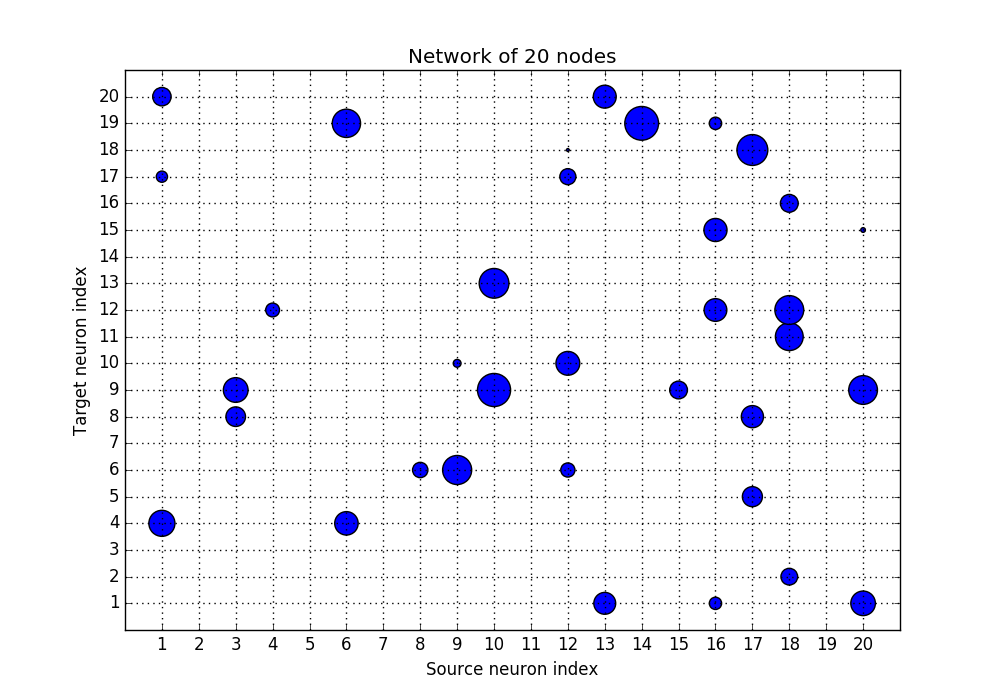
\includegraphics[width=0.8\textwidth]{graph_20_nodes.png}
  \caption{Adjacency matrix of a network of 20 nodes}
	\label{fig:graph_20_nodes}
\end{figure}

The superscript \textit{BNN} in $\alpha_{j,i}^{BNN}$ is employed to differentitate between the weights in biological neural networks and the analogous transmission rates $\alpha_{j,i}$ in diffusion networks \cite{pranav_report}. When neurons $j$ and $i$ are connected with a weight $\alpha_{j,i}^{BNN}$, everytime $j$ spikes, it causes the membrane potential $v$ from Eq.\ref{eq:izhikevich_ode} to increase by $\alpha_{j,i}^{BNN}$. If neuron $i$ crosses the threshold of 30mV, it spikes. This phenomenon is proved in \cite{alexandru2018estimating} and explained in section \textbf{insert reference}. Using the example in figure \ref{fig:graph_20_nodes}, when node 10 spikes, it causes nodes 13 and 9 to increase by $\alpha_{10,13}^{BNN}$ and $\alpha_{10,9}^{BNN}$, respectively. 


The type of networks that were simulated in \cite{alexandru2018estimating} are generated by Erdös \& Reny random graphs, where each possible edge in the network has an independent probability $p$ of being present. The weights assigned to the edges are the output of a uniform distribution in (0,30], the threshold value in Eq.\ref{eq:izhikevich_ode}. It can be observed that the adjacency matrix does not contain weights where $i=j$ because spikes do not increase the membrane potential of the source neuron.


\subsubsection{Input stimulus model for cascade generation}

The neurons in the brain are susceptible to input stimuli from the rest of the neurons in the network. This is represented in the Izhikevich neuron model with the $I$ component in Eq.\ref{eq:izhikevich_ode}. This term can be employed to model injected current in the form of a DC input or can be normally distributed\footnote{In the Izhikevich neuron model \cite{izhikevich2003simple}, the mean and standard deviation are equal to 0 and 5 for excitatory neurons and to 0 and 2 for inhibitory neurons, respectively.} to represent noise from interactions with neurons that are outside the network being recorded.

The selection of an appropriate input stimulus for the neurons was a challenge encountered by Malhotra \cite{alexandru2018estimating}. With a Gaussian input $I$, neurons spike at random times and there is no systematic way of selecting the beginning of a cascade. In a cascade where nodes 1, 3 and 5 spike in chronological order, each of them could have in turn their own cascade (i.e 1, 3 and 5; 3 and 5; and 5). However, this breaks the requirement of independence of cascades seen in section \ref{sec:diffusion_processes}, where no same spike can appear in two cascades. For this reason, a well studied approach was required for the selection of cascades. 

The solution Malhotra found to this problem was to provide one neuron at a time with a constant input of 12 and the rest of the neurons with Gaussian noise. This caused the selected neuron to spike periodically. With an appropriate selection of the DC input, the spiking frequency could be changed, and with a sufficiently long time between spikes, the network could settle into a steady state. Unlike infections in diffusion networks, neurons can spike more than once. For this reason the horizon was arbitrarily limited so as to not allow two spikes from the same cascade to occur in the same cascade and, therefore, obey the law of binary infections imposed by NetRate \cite{alexandru2018estimating}.

This method provides a systematic way of generating cascades: every time the node with DC input spiked, a new independent cascade was created. In order to obtain cascade information from all the nodes in the network, all nodes are stimulated over the course of an experiment. Otherwise, if only one node was selected, no information would be extracted from the nodes with no direct connection to it \cite{pranav_report}. 

The experimental results obtained by Malhotra show that an optimal amount of spiking information that achieves a high inferring performance is achieved with a stimulation time of 4,000 ms. This is due to the underlying probabilistic nature of NetRate \cite{pranav_report}. In other words, more data does not result in a higher performance.

\subsubsection{Likelihood function}

The ability of NetRate to infer the weights in the adjacency matrix \textbf{A} stems from the fact that the shape of $f(t_{i}\mid t_{j};a_{j,i})$ provides a probabilistic description of $\alpha_{j,i}$. The Izhikevich spiking neuron is modelled deterministically while the propagation of infections is probabilistic. For this reason the suitability of NetRate for the biological network inference was proved in \cite{alexandru2018estimating}.

As was explained in section \ref{sec:cascade_generation}, it is not possible to determine exactly which node caused some other node to become infected. However, this is not true for the Izhikevich neuron spikes. It was shown in \cite{alexandru2018estimating} that 




\newpage
\printbibliography 


\end{document}









